\documentclass[a4paper,12pt]{report}

\usepackage[utf8x]{inputenc}
\usepackage[T2A]{fontenc}
\usepackage[english, russian]{babel}

% Опционно, требует  apt-get install scalable-cyrfonts.*
% и удаления одной строчки в cyrtimes.sty
% Сточку не удалять!
% \usepackage{cyrtimes}

% Картнки и tikz
\usepackage{graphicx}
\usepackage{tikz}
\usetikzlibrary{snakes,arrows,shapes}


% Увы, поля придётся уменьшить из-за листингов.
\topmargin -1cm
\oddsidemargin -0.5cm
\evensidemargin -0.5cm
\textwidth 17cm
\textheight 24cm

\sloppy



% Оглавление в PDF
\usepackage[
bookmarks=true,
colorlinks=true, linkcolor=black, anchorcolor=black, citecolor=black, menucolor=black,filecolor=black, urlcolor=black,
unicode=true
]{hyperref}

% Для исходного кода в тексте
% \newcommand{\Code}[1]{\texttt{#1}}

% Некоторая русификация.
% \usepackage{misccorr} % Oh shi^W^W, оно не работает с report.
\usepackage{indentfirst}
\renewcommand{\labelitemi}{\normalfont\bfseries{--}}

% На дворе XXI век, но пакет listings всё ещё не пашет с русскими комментариями!

% Пакет listings для простой вставки исходников
% \usepackage{listings}
% Параметры оформления
% \lstset{
% showspaces=false,
% showtabs=false,
% frame=single,
% tabsize=4,
% basicstyle=\ttfamily,
% identifierstyle=\ttfamily,
% commentstyle=\itshape,
% stringstyle=\ttfamily,
% keywordstyle=\ttfamily,
% breaklines=true
% }
% Русский в комментариях.
% \lstset{escapebegin=\begin{cyr},escapeend=\end{cyr}}



% А это взято из файла, сгенерённого doxygen
\usepackage{calc}
\usepackage{array}
\newenvironment{Code}
{\footnotesize}
{\normalsize}
\newcommand{\doxyref}[3]{\textbf{#1} (\textnormal{#2}\,\pageref{#3})}
\newenvironment{DocInclude}
{\footnotesize}
{\normalsize}
\newenvironment{VerbInclude}
{\footnotesize}
{\normalsize}
\newenvironment{Image}
{\begin{figure}[H]}
{\end{figure}}
\newenvironment{ImageNoCaption}{}{}
\newenvironment{CompactList}
{\begin{list}{}{
  \setlength{\leftmargin}{0.5cm}
  \setlength{\itemsep}{0pt}
  \setlength{\parsep}{0pt}
  \setlength{\topsep}{0pt}
  \renewcommand{\makelabel}{\hfill}}}
{\end{list}}
\newenvironment{CompactItemize}
{
  \begin{itemize}
  \setlength{\itemsep}{-3pt}
  \setlength{\parsep}{0pt}
  \setlength{\topsep}{0pt}
  \setlength{\partopsep}{0pt}
}
{\end{itemize}}
\newcommand{\PBS}[1]{\let\temp=\\#1\let\\=\temp}
\newlength{\tmplength}
\newenvironment{TabularC}[1]
{
\setlength{\tmplength}
     {\linewidth/(#1)-\tabcolsep*2-\arrayrulewidth*(#1+1)/(#1)}
      \par\begin{tabular*}{\linewidth}
             {*{#1}{|>{\PBS\raggedright\hspace{0pt}}p{\the\tmplength}}|}
}
{\end{tabular*}\par}
\newcommand{\entrylabel}[1]{
   {\parbox[b]{\labelwidth-4pt}{\makebox[0pt][l]{\textbf{#1}}\vspace{1.5\baselineskip}}}}
\newenvironment{Desc}
{\begin{list}{}
  {
    \settowidth{\labelwidth}{40pt}
    \setlength{\leftmargin}{\labelwidth}
    \setlength{\parsep}{0pt}
    \setlength{\itemsep}{-4pt}
    \renewcommand{\makelabel}{\entrylabel}
  }
}
{\end{list}}
\newenvironment{Indent}
  {\begin{list}{}{\setlength{\leftmargin}{0.5cm}}
      \item[]\ignorespaces}
  {\unskip\end{list}}


\title{Расчетно-Пояснительная Записка \\
    \large к курсовой работе на тему: \\ Серверная часть MTA SMTP}
\author{Сычев С.А. ИУ7-32М}

\begin{document}

\maketitle

\tableofcontents

\newpage
\chapter*{Введение}
\addcontentsline{toc}{chapter}{Введение}

Данная работа посвящена разработке серверной части почтового сервера MTA (англ. Message Transfer Agent), использующего протокол SMTP (англ. Simple Mail Transfer Protocol) - сетевой протокол, предназначенный для передачи электронной почты в сетях TCP/IP. 

Цель работы: спроектировать, разработать и протестировать серверную часть почтового SMTP-сервера (MTA), обеспечивающую локальную доставку сообщений и их добавление в очередь удаленной доставки. 

Дополнительные условия:
\begin{itemize}
\item Использовать системный вызов \texttt{poll()};
\item Использовать рабочие процессы;
\item Журналирование осуществлять в отдельном процессе.
\item Требуется проверять обратную зону DNS.
\end{itemize}

Для достижения цели работы, необходимо выполнить следующие задачи:
\begin{enumerate}
    \item Изучить и проанализировать предметную область, достоинства и недостатки требуемого способа разделения на процессы и опроса сокетов;
    \item Спроектировать серверную часть MTA SMTP;
    \item Реализовать серверную часть MTA SMTP; 
    \item Отладить и протестировать серверную часть MTA SMTP
\end{enumerate}

\newpage
\chapter{Аналитический раздел}

\section{Протокол SMTP}
SMTP ~-- это сетевой протокол, предназначенный для передачи писем электронной почты в сетях TCP/IP. SMTP впервые был описан в RFC 821 (1982 год), а последнее обновление описано в RFC 5321 [1] и включает масштабируемое расширение протокола — ESMTP (Extended SMTP). В настоящее время под протоколом SMTP подразумеваются и его расширения. Протокол SMTP предназначен для передачи исходящей почты с использованием порта TCP 25.

Взаимодействие в рамках SMTP строится по принципу двусторонней связи, устанавливаемой   между отправителем и получателем почтового сообщения. При этом отправитель инициирует соединение и посылает запросы, а получатель - отвечает на эти запросы. Таким образом, отправитель выступает в роли клиента, а получатель - сервера.

\subsection{Команды протокола SMTP}

Команды протокола SMTP начинаются с названий - ключевых слов, указывающих, какую операцию хочет осуществить клиент.
За ключевым словом следуют, отделенные пробелом, параметры. Конец команды обозначается последовательностью символов \textbackslash r\textbackslash n - обозначаемой CRLF. 

Ниже представлен список базовых SMTP-команд:
\begin{itemize}
	\item \textbf{HELO [доменное имя клиента] CRLF} - Открывает SMTP сессию. В RFC 2821 рекомендуется использовать команду HELO, только если программное обеспечение не поддерживает команду EHLO.
	\item \textbf{EHLO [доменное имя клиента] CRLF} - Открывает ESMTP сессию. В ответ на эту команду сервер сообщает, готов ли он к продолжению диалога.
	\item \textbf{MAIL FROM: <адрес\_отправителя> CRLF} - Сообщает адрес отправителя письма. Команда MAIL должна быть выполнена для письма только один раз и только после успешного выполнения команды EHLO или HELO.
	\item \textbf{RCPT TO: <адрес\_получателя> CRLF} - Сообщает адрес получателя письма. Доставка сообщения возможна, только если указан хотя бы один адрес получателя. Команда RCPT может быть выполнена только после успешного выполнения команды MAIL и должна быть повторена для каждого получателя письма.
	\item \textbf{DATA CRLF} - Сообщает о готовности ввода текста письма. Команда DATA может быть выполнена только после успешного выполнения хотя бы одной команды RCPT. После успешного ответа сервера, клиент начинает передачу текста письма, с учетом заголовков. Сервер определяет окончание текста письма по последовательности: CRLF . CRLF
	\item \textbf{RSET CRLF} - Сброс SMTP соединения. Команда RSET аннулирует все переданные до нее на сервер данные.
	\item \textbf{VRFY <адрес> CRLF} - Проверяет наличия указанного в качестве аргумента почтового адреса.
	\item \textbf{QUIT CRLF} - Закрывает SMTP сессию.
\end{itemize}

Существуют также и другие команды ESMTP, однако в данной работе они не рассматриваются. 

\subsection{Ответы SMTP сервера}

Ответ SMTP сервера состоит из кода ответа, за которым через пробел следует дополнительный текст. Код служит индикатором состояния сервера и делится на четыре группы:
\begin{itemize}
	\item \textbf{2xx} - команда выполнена успешно;
	\item \textbf{3xx} - ромежуточный положительный результат. Команда принята, но сервер ожидает от клиента дополнительные данные для завершения операции;
	\item \textbf{4xx} - исполнение команды временно невозможно. Команда не может быть выполнена, но проблема может быть устранена;
	\item \textbf{5xx} - исполнение команды невозможно.
\end{itemize}

Если ответ сервера состоит из нескольких строк, то каждая из них начинается кодом, который отделяется от сопровождающего текста не пробелом, а символом "минус"\ (-). В последней строке номер отделяется от текста пробелом. Каждая строка ответа, как и строки команд, заканчивается последовательностью CRLF.

\section{Преимущества и недостатки использования системного вызова poll.}

Системный вызов poll, по сравнению с другими системными вызовами опроса сокетов имеет следующие достоинства [2]: 
\begin{itemize}
	\item Отсутствие активного ожидания на процессоре.
	\item Обрабатка больше 1024 клиентов по сравнению с системным вызовом \texttt{select()}.
	\item Не модифицируется структура pollfd, что даёт возможность её переиспользования между вызовами poll() — нужно лишь обнулить поле revents.
	\item Наблюдаемые события лучше структурированы. Например, можно определить отключение удалённого клиента без необходимости чтения данных из сокета.
\end{itemize}

К его недостаткам можно отнести [2]:
\begin{itemize}
 	\item Poll отсутствует на некоторых платформах (в основном старых). 
	\item Невозможнось определить, какие именно дескрипторы сгенерировали события, без полного прохода по всем наблюдаемым структурам и проверки поля revents. (Проблема так-же в том, что в ядре данная операция реализована так-же). 
	\item Как и при использовании select, нет возможности динамически менять наблюдаемый набор событий. 
\end{itemize}

\section{Преимущества и недостатки использования нескольких рабочих процессов.}

Использование нескольких рабочих процессов имеет следующие преимущества:
\begin{itemize}
	\item Позволяет повысить возможности сервера по одновременной обработке нескольких клиентов. 
	\item Позволяет освободить высоконагруженные процессы, работающие с клиентами некоторых "тяжелых" задач, таких как операции файлового ввода/вывода. 
	\item Позволяет более полно использовать возможности современных многоядерных процессоров. 
\end{itemize}

К недостаткам использования многопроцессности можно отнести:
\begin{itemize}
	\item повышение сложности разработки за счет необходимости корректного завершения всех процессов, ожидания, а также межпроцессного взаимодействия. 
	\item Как и при использовании select, нет возможности динамически менять наблюдаемый набор событий. 
\end{itemize}

\section{Сущности предметной области}

Для серверной части SMTP MTA можно выделить следующие основные сущности предметной области: 
\begin{enumerate}
	\item клиент (подключение) - это текущее активное соединение клиента с сервером, к нему можно отнести буферы ввода вывода и текущее состояние. 
	\item письмо - получаемое от клиента сообщение, содержащее информацию от отправителе и получателях, имеющее заголовки и тело.  
	\item почтовый адрес - это почтовый адрес, получатель, или один из отправителей письма. 
\end{enumerate}

ER-диаграмма сущностей предметной области приведена на \ref{fig:er}

\begin{figure}[H]
	\centering
	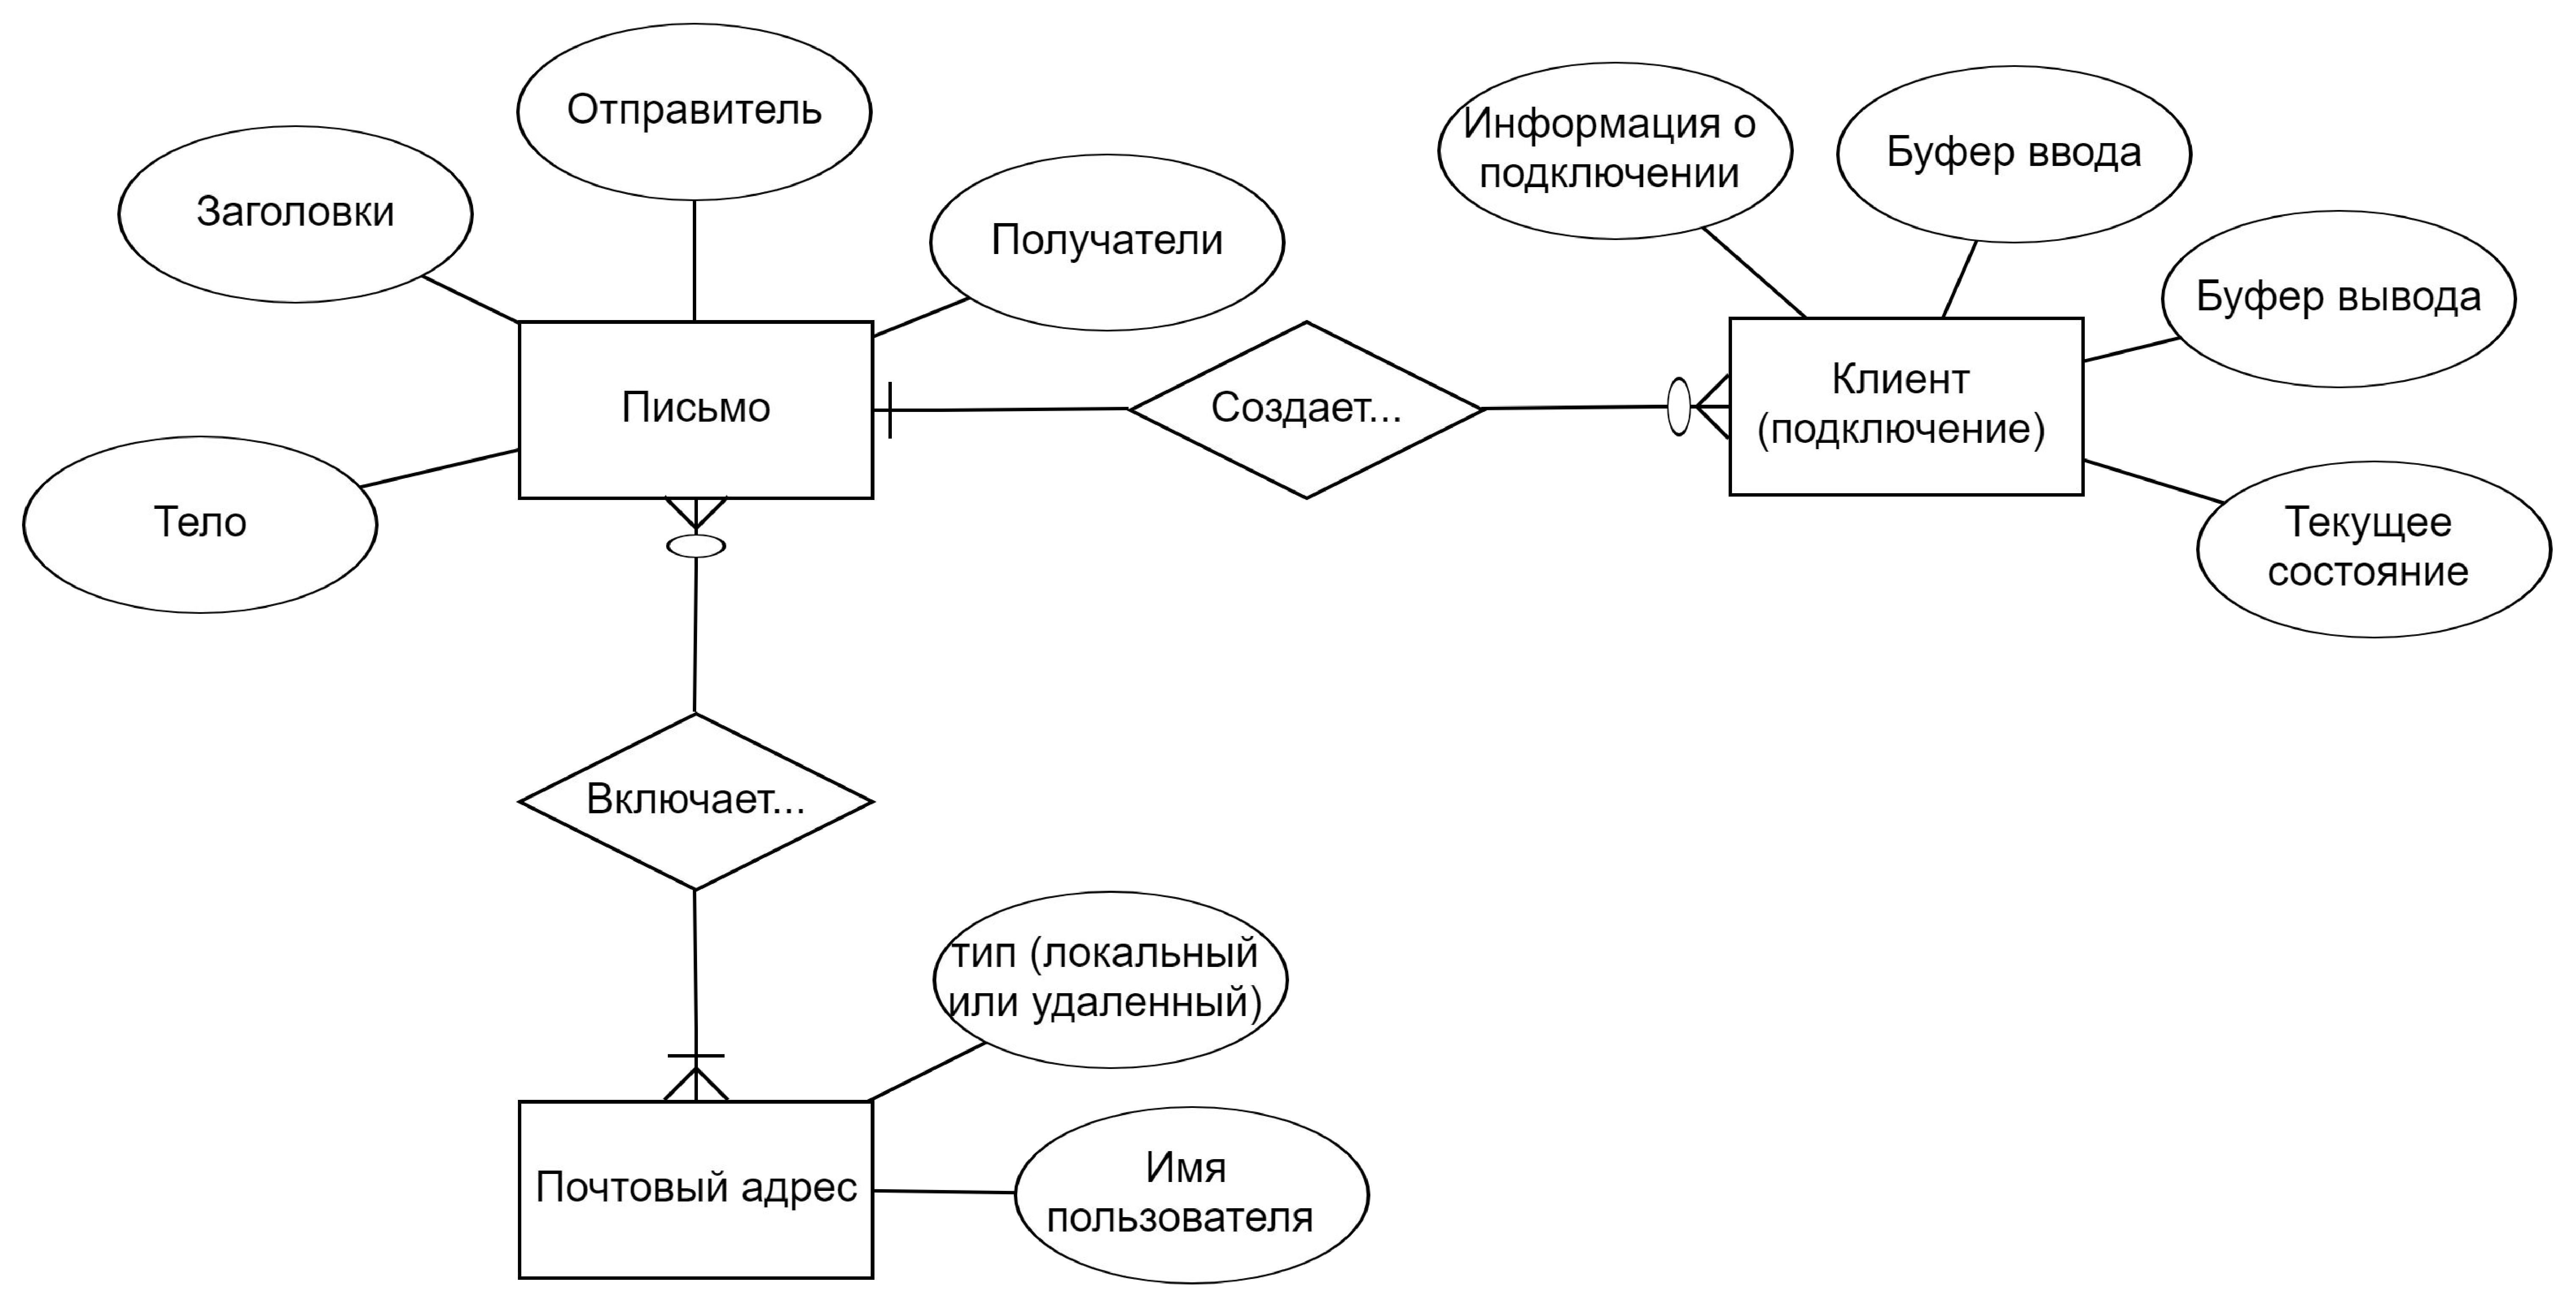
\includegraphics[width=0.7\textwidth]{include/er.pdf}
	\caption{ER-диаграмма сущностей предметной области}
	\label{fig:er}
\end{figure}

\newpage
\chapter{Конструкторский раздел}

\section{Описание основных структур данных}

В результате проектирования системы, были получены следующие основные структуры данных: 
\begin{itemize}
	\item \textbf{server} - абстракция сервера, содержащая в себе все, что требуется для обработки соединений в одном потоке выполнения. 
	\item \textbf{logger} - абстракция логгера, содержащая все необходимые структуры данных для работы логгера или отправки данных в логгер. 
	\item \textbf{client\_info} - абстракция информации о клиенте, содержит статус, буферы ввода вывода и другую информацию о клиенте.
	\item \textbf{mail} - абстракция письма, содержит адрес отправителя, адреса получателей и текст письма. 
	\item \textbf{string} - абстракция строки, предоставляет ряд удобных функций по работе со строками. Осуществляет автоматическое перевыделение памяти, в случае необходимости. 
	\item \textbf{address} - абстракция адреса, соредрит строку адреса, а также его тип. 
	\item \textbf{process\_info} - абстакция процесса, содержит информацию о процессе и его потомках, необходимую для корректного завершения программы. 
	\item \textbf{server\_parser} - абстракция обработчика входного буфера. 
	\item \textbf{server\_parser\_result} - абстракция результата работы парсера. 
	\item \textbf{compiled\_regexp} - абстракция скомпилированного регулярного выражения. 
\end{itemize}

На \ref{fig:uml} приведена UML-диаграмма основных структур данных.

\begin{figure}[H]
	\centering
	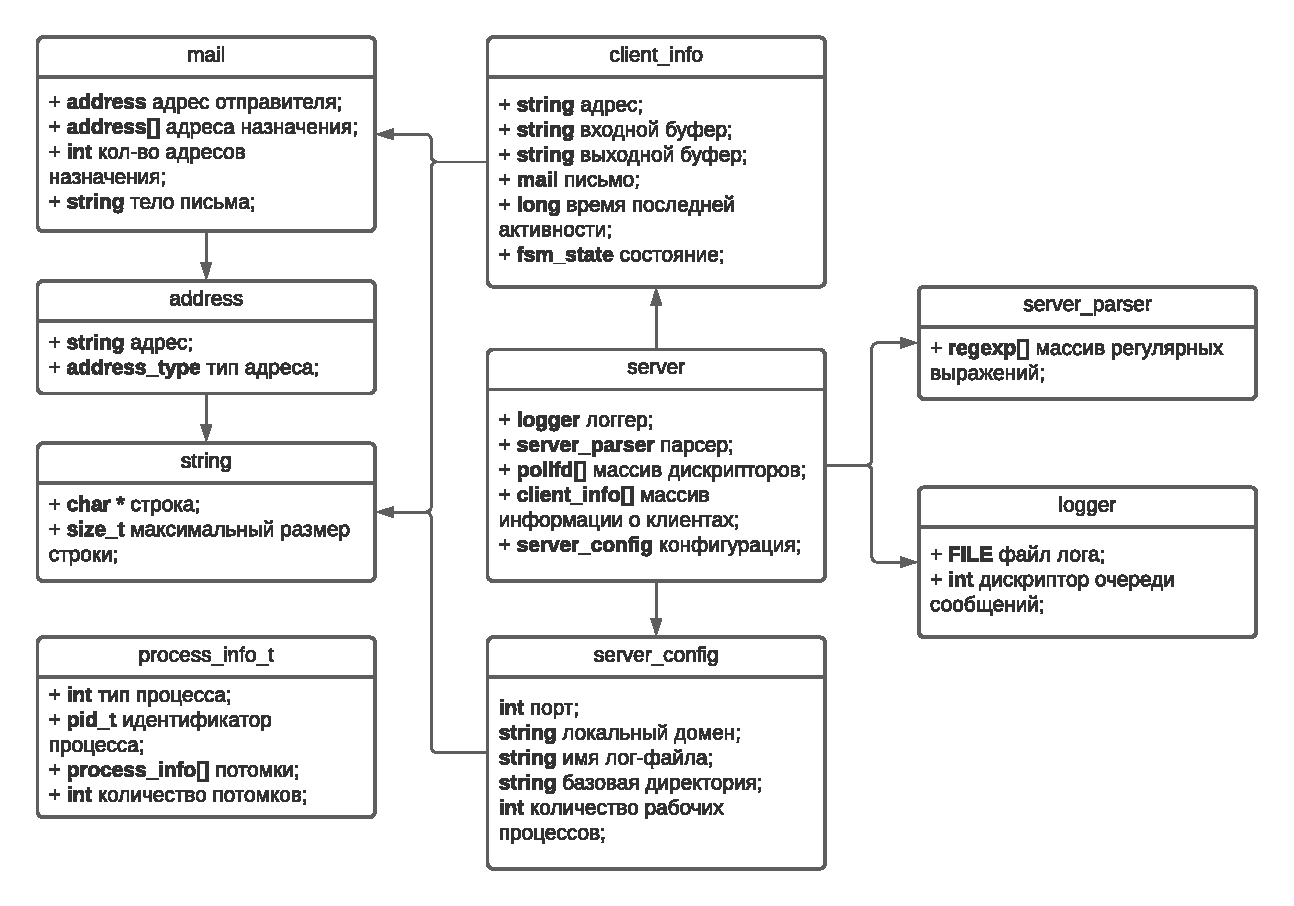
\includegraphics[width=\textwidth]{include/uml.pdf}
	\caption{Диаграмма основных структур данных}
	\label{fig:uml}
\end{figure}

\section{Обработка соединений в одном потоке выполнения}

Ниже привезен псевдокод обработки соединений в одном потоке выполнения: 
\begin{lstlisting}
	Основной цикл обработки:
		poll:
			Если пришло сообщение в дескриптор сигнала выхода:
				Завершить работу сервера, закрыв все клиентские сокеты
	
			Если пришло сообщение на слушающий сокет сервера:
				Добавить нового клиента (обработав подключение)
				Начать новую итерацию цикла (continue)
	
			Цикл по всем дескрипторам клиентских сокетов:
				Если на сокет клиента пришло сообщение:
					Обнулить таймер клиента
					Обработать сообщение от клиента
					Начать новую итерацию цикла (continue)
				Если есть неотправленное сообщение для клиента: 
					Отослать сообщение клиенту
					Начать новую итерацию цикла (continue)	
					
		Цикл по всем подключенным клиентам:
			Если таймер клиента превысил определенное значение:
				Отправить клиенту сообщение об истечении таймера
			Eсли произошла внутренняя ошибка: 
				Отправить клиенту сообщение об ошибке
			Если сессия с клиентом завершена:
				Очистить данные о клиенте
				Закрыть соединение с клиентом
\end{lstlisting}

\section{Распределение задач по процессам}

В данной работе предполагается использование фиксированного количества рабочих процессов. При этом по условию задания - журналирование также должен осуществлять отдельный процесс. 

Основная задача SMTP сервера - обрабатывать подключающихся клиентов, сохраняя письма, присылаемые ими. Данная задача может выполняться в нескольких процессах параллельно. При этом, если каждого отдельного клиента, процесс обрабатывает полностью самостоятельно, не потребуется какого-либо взаимодействия. 

Таким образом, разницы с точки зрения выполняемого серверного кода для основного родительского процесса и его потомков нет. Единственным отличием родительского процесса является то, что при завершении работы программы, он должен корректно дождаться завершения всех своих потомков. 

Таким образом, SMTP сервер создает процессы следующих видов, со следующими задачами:
\begin{enumerate}
	\item MASTER - родительский процесс, создающий остальных, после чего выполняющий основной серверный код и обрабатываюший подключающихся клиентов. При завершении работы программы ожидает завершения своих потомков. 
	\item WORKER - дочерний процесс, выполняющий основной серверный код и обрабатываюший подключающихся клиентов.  
	\item LOGGER - дочерний процесс журналирования, выполняет непосредственную запись логов в файл и консоль. 
\end{enumerate}

На рис.~\ref{fig:processes} синими стрелками отмечены отношения типа родитель-потомок между процессами. 

\section{Межпроцессное взаимодействие}

В силу того, что отдельные клиенты обрабатываются в отдельных процессах изолировано, межпроцессное взаимодействие необходимо только для передачи логов процессу журналирования. 
На рис.~\ref{fig:processes} черными прерывистыми линиями показана передача данных от процессов друг другу. 

\begin{figure}[H]
	\centering
	\includegraphics[width=\textwidth]{build/processes.pdf}
	\caption{Диаграмма межпроцессного взаимодействия}
	\label{fig:processes}
\end{figure}

Для передачи логов используются очереди сообщений и системные вызовы msgrcv msgsend и др. 

Родительский процесс, создавая процесс журналирования, перед дальнейшей работой, ожидает от него подтверждения готовности (сообщение особого типа). После чего, в очередь сообщений отправляются логи. 

Для остановки процесса журналирования также используется сообщение специального типа, отправляемое родительским процессом.

Рабочим процессам не требуется отдельно передавать сигнал завершения, так как они наследуют от родительского файловый дискриптор для получения этого сигнала, и получат сигнал без каких либо дополнительных действий. 

\section{Конечный автомат состояний сервера}

На рис.~\ref{fig:fsm} изображен конечный автомат разрабатываемой серверной части SMTP сервера. 

\begin{figure}[H]
	\centering
	\includegraphics[width=\textwidth]{build/fsm.pdf}
	\caption{Конечный автомат состояний сервера}
	\label{fig:fsm}
\end{figure}

\section{Регулярные выражения для парсинга SMTP команд}

Регулярные выражения для парсера SMTP команд приведены на листинге ниже: 

\lstinputlisting[caption=parser/server\_parser.h, firstline=12,lastline=66]{../../src/parser/server_parser.h}

\section{Хранение почты}

Для хранения локальной почты, то есть почты, предназначенной для клиентов с почтовым доменом сервера, используется формат Maildir. Maildir - формат хранения электронной почты, не требующий монопольного захвата файла для обеспечения целостности почтового ящика при чтении, добавлении или изменении сообщений. Каждое сообщение хранится в отдельном файле с уникальным именем. Вопросами блокировки файлов при добавлении, перемещении и удалении файлов занимается локальная файловая система. Все изменения делаются при помощи атомарных файловых операций, таким образом, монопольный захват файла ни в каком случае не нужен.

Путь до директории с письмами, адресованными пользователю user будет выглядеть следующим образом:
\begin{lstlisting}
	base_maildir/user/maildir/new/
\end{lstlisting}

Для хранения почты, преднозначенной другим почтовым серверам также используется формат Maildir. Единственное отличие - отсутствие в пути к файлу имени клиента т.е.: 
\begin{lstlisting}
	base_maildir/maildir/new/
\end{lstlisting}

Имена файлов с письмами генерируюстя также в соответствии с Maildir и содержат случайное число, текущее время (UNIX Time) и префикс сервера. 

Ниже приведен пример такого имени: 
\begin{lstlisting}
	1610708049.10777.smtp_serv.846930886:2,
\end{lstlisting}

\chapter{Технологический раздел}

\section{Язык программирования и библиотеки}

Для написания исходного кода SMTP сервера использовался язык C стандарта C99.

Помимо стандартных библиотек были использованы:
\begin{itemize}
    \item libconfig - библиотека для чтения файлов конфигурации [3].  
    \item Autogen - библиотека для автоматической генерации конечного автомата состояний.
    \item PCRE - библиотека для работы с регулярными выражениями [4]. 
    \item CUnit - библиотека для модульного тестирования [5].
\end{itemize}


\section{Платформы и компиляторы}

Для сборки использовался компилятор gcc, со следующими флагами: 
\begin{lstlisting}
-std=c99 -g -g3 -O0 -Wall -Werror -pedantic -D\_GNU\_SOURCE
\end{lstlisting}
Программное обеспечение разрабатывалось, собиралось и тестировалось на виртуальной машине с ОС Ubuntu 16.04, с двухядерным процессором и 4 ГБ оперативной памяти. 


\section{Сборка}
Сборка осуществляется при помощи утилиты Make. Применен иерархический подход. Сценарии сборки описаны в трех Makefile-ах. 
\begin{enumerate}
	\item Makefile для сборки и тестирования сервера - расположен в каталоге \textbf{/server/src} и отвечает за непосредственную сборку и тестирование сервера. 
	\item Makefile для сборки отчета - расположен в каталоге \textbf{/server/report} и отвечает за сборку данного отчета. 
	\item Корневой Makefile - расположен в каталоге \textbf{/server}, объединяет функции двух предыдущих, имеет общие цели для сборки сервера, его тестирования и генерации отчета, по итогам тестирования. 	
\end{enumerate}

\section{Визуализация сценариев сборки}
В данном разделе приведена визуализиция Makefile-ов, используемых для сборки и тестирования сервера и отчета. 
Визуализация корневого Makefile-а не приводится так как она во многом повторяет указанные ранее. 
\begin{figure}[H]
	\centering
	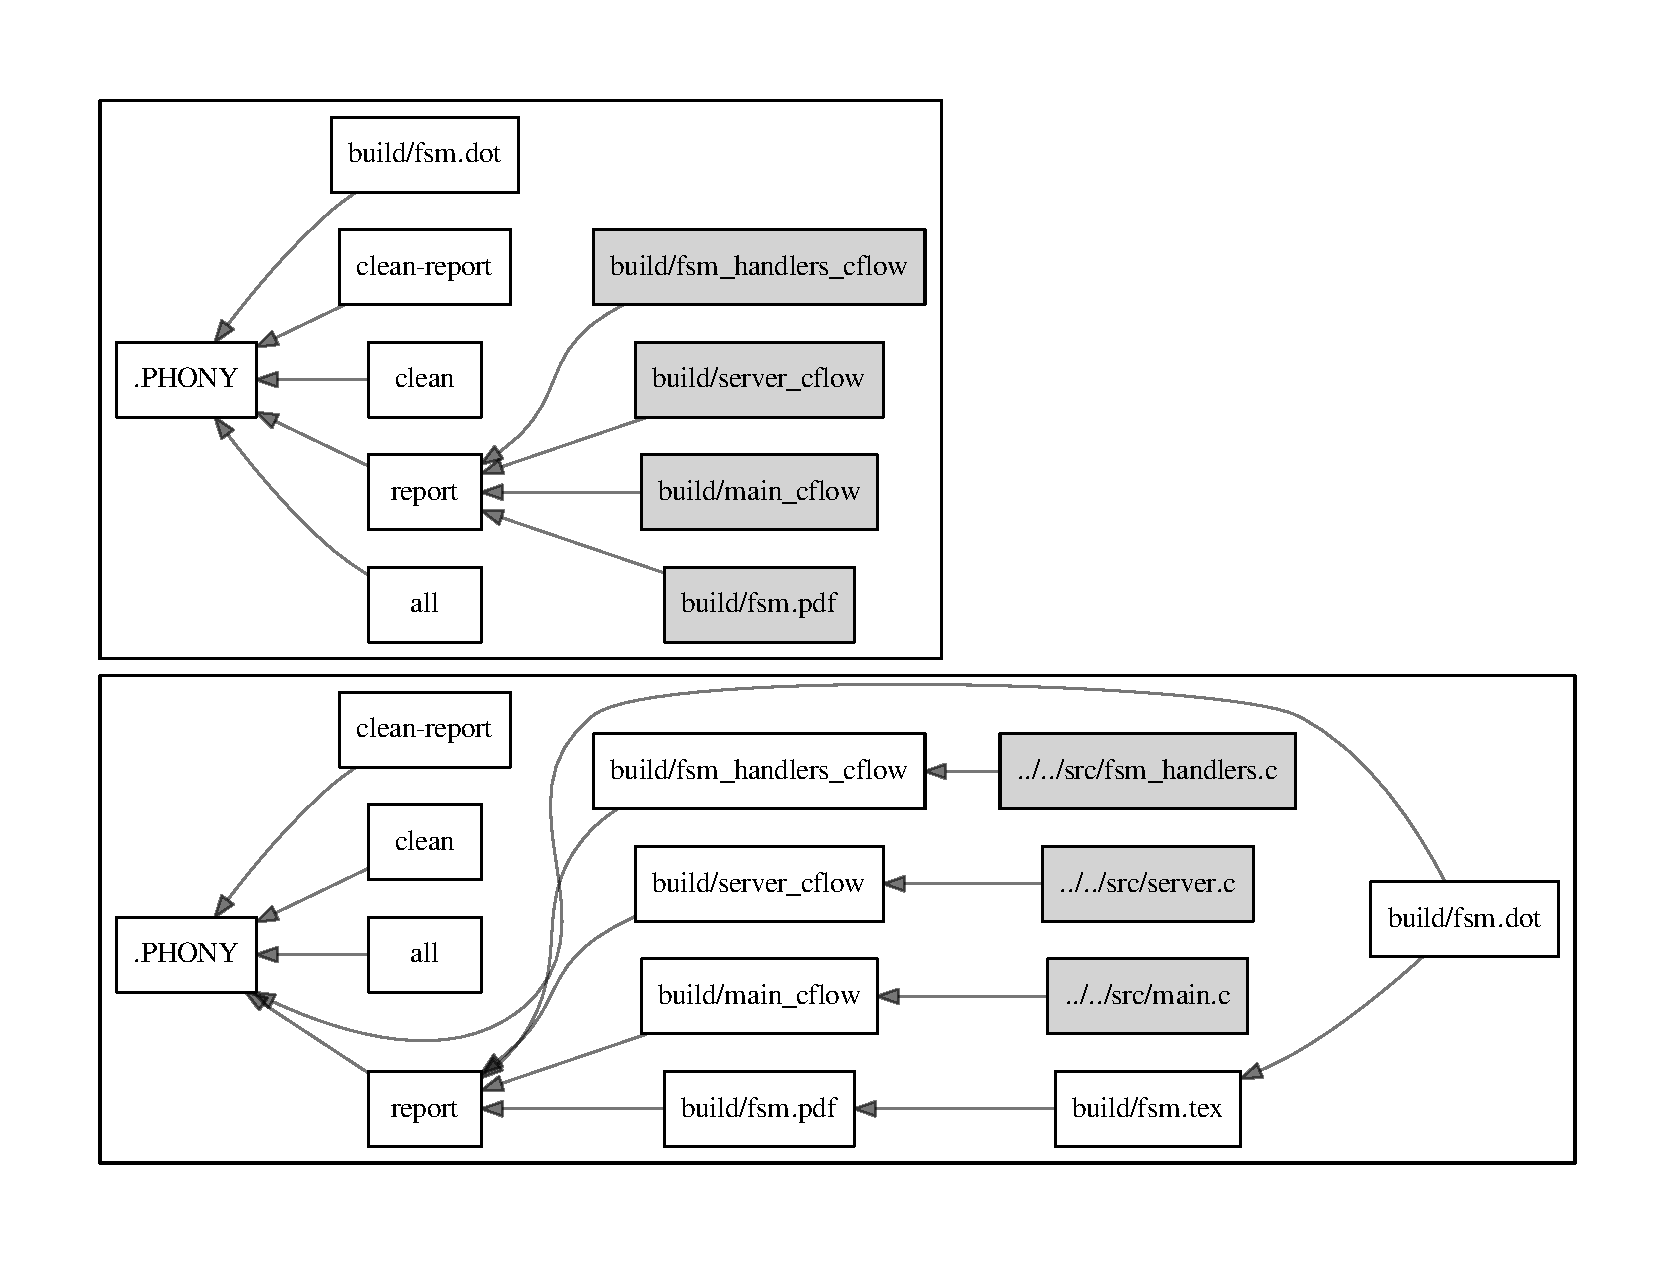
\includegraphics[width=\textwidth]{include/report_make.pdf}
	\caption{Визуализация сценария сборки отчета}
	\label{fig:make2}
\end{figure}

\begin{figure}[H]
	\centering
	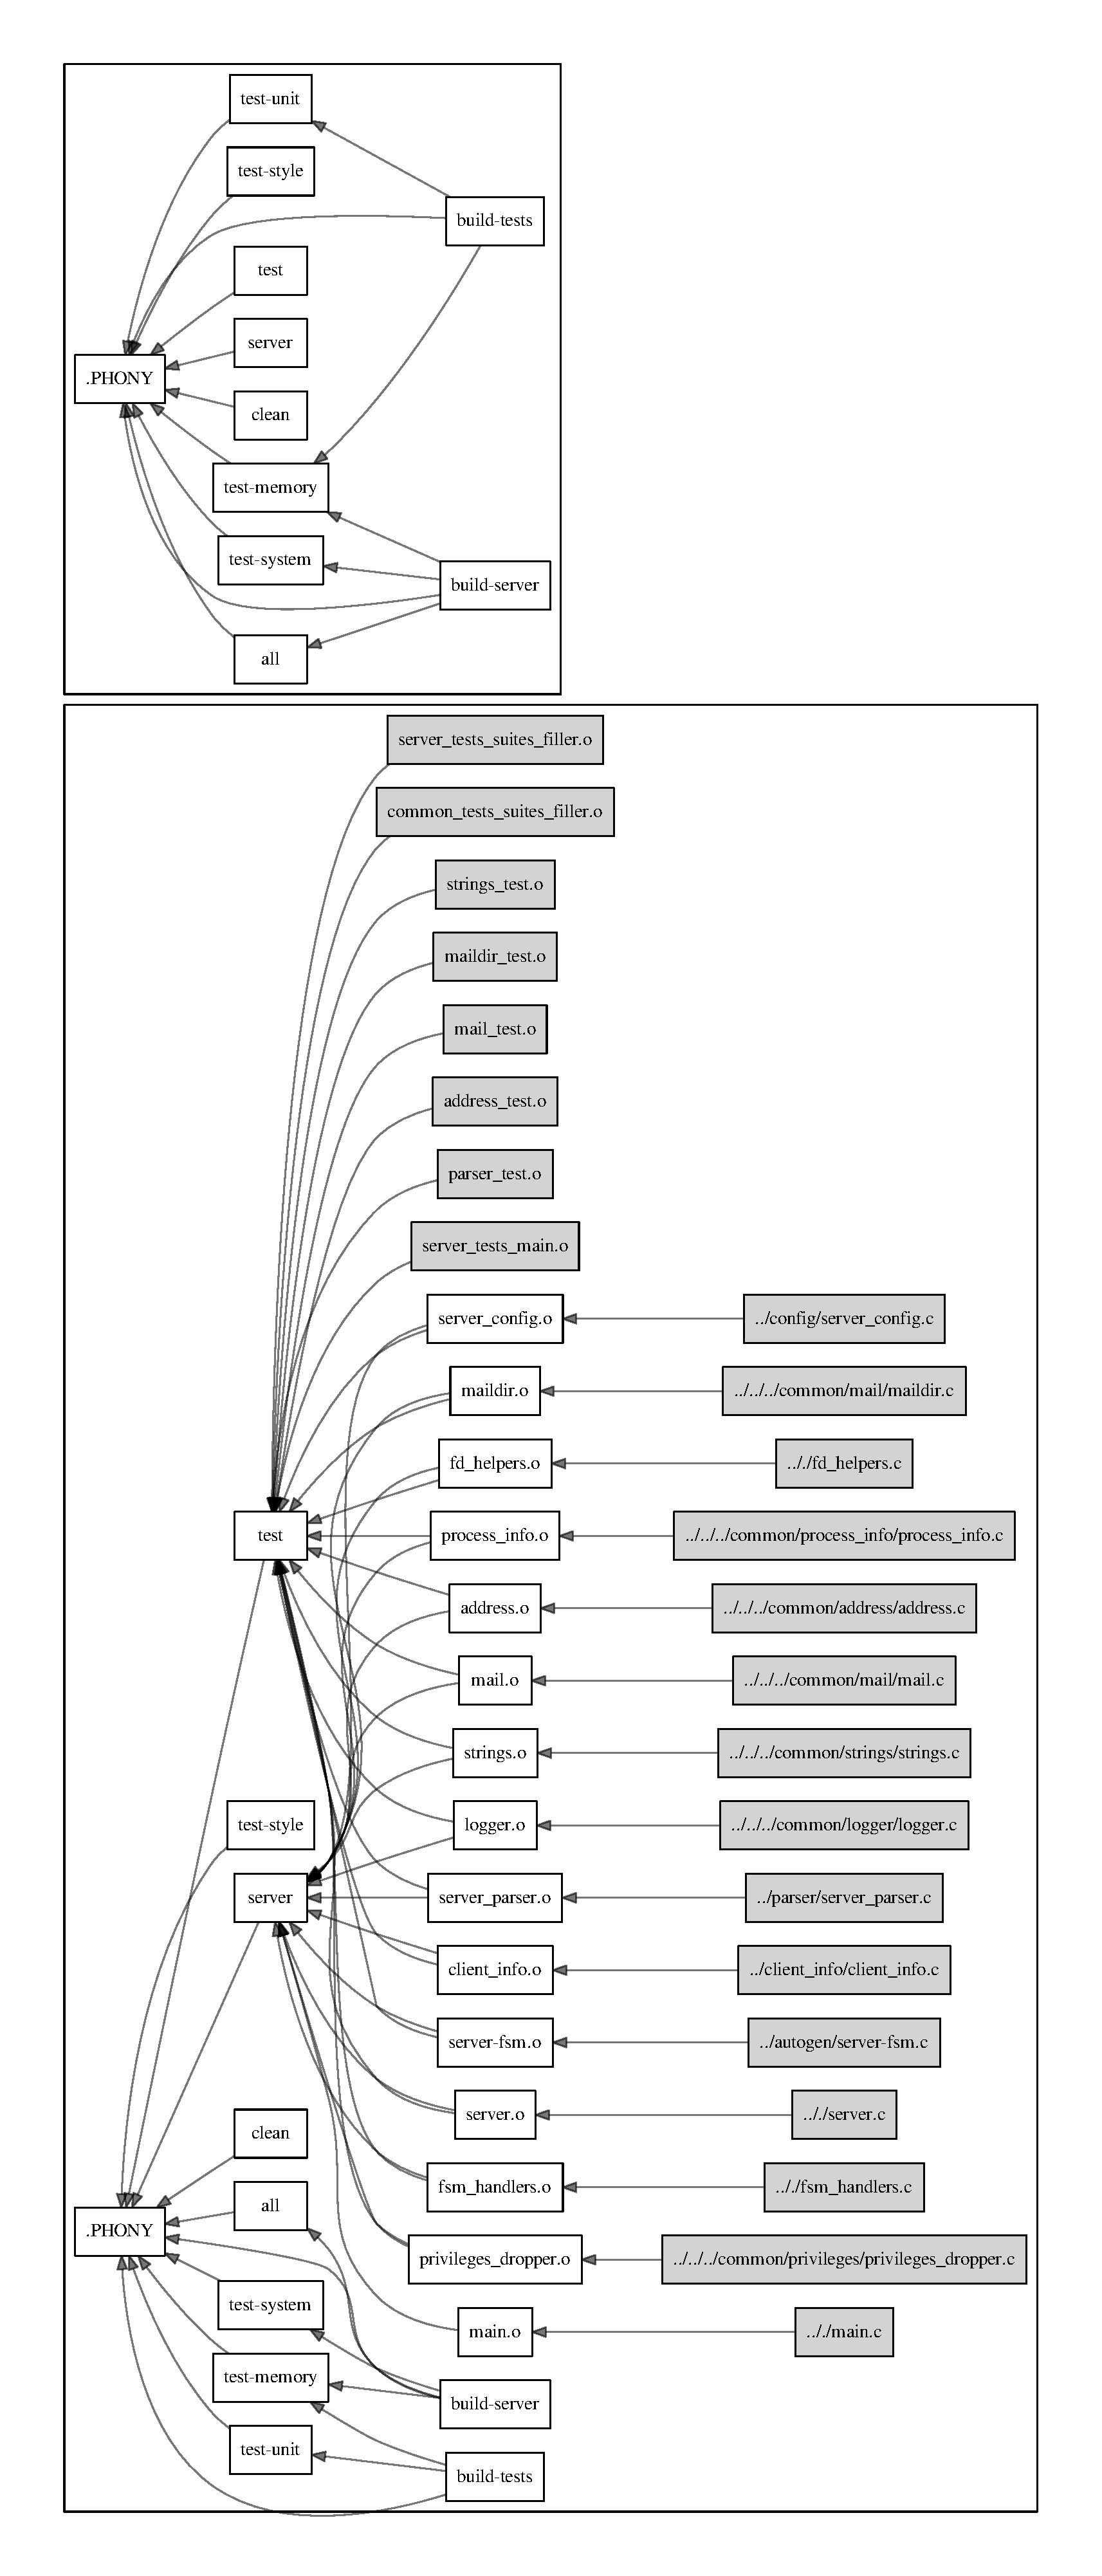
\includegraphics[width=0.65\textwidth]{include/server_make.pdf}
	\caption{Визуализация сценария сборки и тестирования сервера}
	\label{fig:make1}
\end{figure}

\section{Кодогенерация}
Для ускорения разработки конечного автомата сервера была применена библиотека autogen. 

Из .def файла с описанием конечного автомата был сгенерирован код, осуществляющий все переключения между состояниями. 

Далее потребовалось лишь написать обработчики переходов. 

Файл, на основании которого был сгенерирован автомат приведен на листинге ниже:
\lstinputlisting[basicstyle=\tiny]{../../src/autogen/server.def}

\section{Конфигурация}
Для конфигурирования сервера, используется конфигурационный файл, путь до которого необходимо передавать как параметр командной строки при запуске сервера. 

Для чтения файла конфигурации используется библиотека: \textbf{libconfig}.

В файле конфигурации задаются: 
\begin{itemize}
	\item version - версия файла конфигурации, необходима, чтобы отличить новые версии конфига, в случае дальнейшей работы над проектом.  
	\item port - порт, на котором будет слушать сервер.  
	\item local\_domain - почтовый домен, который сервер будет считать локальным (и письма будут записываться в соответствии с maildir).
	\item log\_filename - имя файла с логом. 
	\item maildir - базовая директория для записи писем.
	\item max\_process\_cnt - максимальное количество рабочих процессов (без учета логгера). 
\end{itemize}


Ниже привезен пример файла конфигурации:
\lstinputlisting{../../src/server.ini}

\section{Графы вызова функций}
Ниже приведены графы вызова функций для точки входа (\textit{main.c}), основного серверного кода (\textit{server.c}) и обработчиков переходов состояний (\textit{fsm\_handlers.c}). Из графов для большей наглядности удалены обращения к следующим функциям: 

\lstinputlisting{cflowignore.txt}

\begin{figure}[H]
	\includegraphics[width=0.7\textwidth]{build/main_cflow0.pdf}
	\caption{Граф вызовов. Точка входа}
	\label{fig:cflow1}
\end{figure}

\begin{figure}[H]
	\includegraphics[width=1\textwidth]{build/server_cflow0.pdf}
	\caption{Граф вызовов. Основной код сервера}
	\label{fig:cflow2}
\end{figure}
\begin{figure}[H]
	\includegraphics[width=1\textwidth]{build/fsm_handlers_cflow0.pdf}
	\caption{Граф вызовов. Обработчики переходов состояний}
	\label{fig:cflow3}
\end{figure}

\newpage
\section{Модульное тестирование}
Для модульного тестирования функций сервера в работе используется библиотека CUnit.

Модульными тестами покрыто подавляющее большинство функций из библиотек, размещенных в common, т.к. они широко используются в коде серверной части.

Результаты тестирования привидены на листинге ниже: 
\lstinputlisting{../../src/test-unit.out}

\section{Системное тестирование}
Системное тестирование реализовано в виде скрипта на языке Python. Использован SMTP клиент из стандартной библиотеки Python. 

Все тесты устроены следующим образом: 
\begin{itemize}
	\item Подготавливаются данные для отправки письма/писем. 
	\item SMTP клиент подключается к серверу и выполняет отправку одного или нескольких писем. 
	\item Производится проверка корректности записи писем (вплоть до посимвольной проверки содержимого файла).
\end{itemize}

При этом до запуска тестов, автоматически запускается сервер, а после завершения - отправляется сигнал SIGINT, для корректного завершения работы. 

Реализованы следующие системные тесты: 
\begin{itemize}
	\item Простой тест с отправкой небольшого письма одному получателю.  
	\item Тест с отправкой письма, размером ~1МБ.  
	\item Тест с отправкой письма с несколькими получателями, в т.ч. с локальным/удаленным почтовым доменом.
	\item Тест с отправкой нескольких писем в рамках одной SMTP сессии. 
\end{itemize}

Результаты системного тестирования приведены ниже:
\lstinputlisting{../../src/test-system.out}

\section{Тестирование утечек памяти}
Для тестирования утечек памяти использовалась утилита valgrind.

При выполнении основного сценария сборки и тестирования проводится автоматический запуск модульных и системных тестов под valgrind. 

Результаты проверки модульных тестов приведены на листинге ниже, утечек памяти не обнаружено: 
\lstinputlisting{../../src/test-memory.out}


Результаты проверки системных тестов приведены на листинге ниже, утечек памяти не обнаружено: 
\lstinputlisting{../../src/test-system-memory.out}


\section{Тестирование стиля кодирования}

В качестве стиля кодирования был выбран Google С++ style [https://google.github.io/styleguide/cppguide.html] с несколькими незначительными изменениями. 
 
Для проверки стиля кодирования использовалась утилита от Google с открытым исходным кодом: cpplint.py [6]. 

В утилиту были внесены незначительные изменения (для отмены нескольких правил, которые были сочтены излишними). Также применялся флаг для установки максимальной длины строки в 120 символов, вместо стандартных 80.

В ходе автоматической проверки стилевых ошибок не обнаружено, результаты проверки приведены на листинге ниже: 
\lstinputlisting{../../src/test-style.out}

\clearpage
\chapter*{Заключение}
\addcontentsline{toc}{chapter}{Заключение}

В ходе работы, были выполнены все поставленные задачи, а именно: 

\begin{enumerate}
	\item Изучена и проанализирована предметная область, достоинства и недостатки требуемого способа разделения на процессы и опроса сокетов;
	\item Спроектирована серверная часть MTA SMTP;
	\item Реализована серверная часть MTA SMTP; 
	\item Отлажена и протестирована серверная часть MTA SMTP.
\end{enumerate}

Таким образом, цель работы достигнута. 

\newpage
\chapter*{Список литературы}
\addcontentsline{toc}{chapter}{Список литературы}

\begin{enumerate}
	\item http://www.faqs.org/rfcs/rfc5321.html - RFC 5321 (Спецификация протокола SMTP)
	\item Статья "select/poll/epoll: практическая разница" [Электронный ресурс] Режим досутпа: URL: https://habr.com/ru/company/infopulse/blog/415259/
	\item https://habr.com/ru/post/148948/ - libconfig "Конфигурационные файлы. Библиотека libconfig" 
	\item https://www.pcre.org/ - офф сайт pcre  
	\item http://cunit.sourceforge.net/documentation.html - документация cunit
	\item https://github.com/google/styleguide/tree/gh-pages/cpplint - github cpplint
	
\end{enumerate}

\lstlistoflistings

\end{document}




